% ASRN: Adaptive Sparse Recurrence Network -- preprint for Zenodo
% Author: Alexis Calvario. Text and figures: CC BY 4.0. Code: Apache 2.0.
% Build: latexmk -pdf ASRN_Calvario_2026_en.tex   (figures: python paper/hacer_figuras.py)
% Numbers: results/banco_a100, results/citas, results/citas_a100 (ASRN 1.0) and, as a replication only,
% history/results/banco_a100_pt211. docs/TECHNICAL_REPORT.md is the long version of this preprint.
\documentclass[11pt]{article}
\usepackage[utf8]{inputenc}
\usepackage[T1]{fontenc}
\usepackage{lmodern}
\usepackage[margin=1in]{geometry}
\usepackage{amsmath,amssymb,amsthm}
\usepackage{graphicx}
\usepackage{booktabs}
\usepackage{xcolor}
\usepackage[numbers,sort&compress]{natbib}
\usepackage{microtype}
\usepackage{caption}
\usepackage{enumitem}
\usepackage[hidelinks]{hyperref}

\captionsetup{font=small,labelfont=bf}
\setlist{itemsep=2pt,topsep=4pt}
\graphicspath{{figuras/en/}}

% Zenodo DOI: fill in after reserving it on Zenodo ("Reserve DOI"); leave empty to omit.
\def\zenododoi{10.5281/zenodo.23607506}

\newcommand{\B}{B}
\newcommand{\Nset}{\mathcal{N}}
\DeclareMathOperator{\softplus}{softplus}
\DeclareMathOperator{\LN}{LN}
\DeclareMathOperator{\GELU}{GELU}
\DeclareMathOperator{\softmax}{softmax}

\title{\textbf{ASRN: Adaptive Sparse Recurrence Networks}\\[4pt]
\large Linear-memory long-range copying with a learned proper-time clock\\ and a Hawkes-gated copy gate}
\author{Alexis Calvario\\ \small Independent researcher\\ \small ORCID: \href{https://orcid.org/0009-0004-0854-6398}{0009-0004-0854-6398}}
\date{\small Preprint, version 1.0 --- October 2026%
\ifx\zenododoi\empty\else\\ DOI: \href{https://doi.org/\zenododoi}{\zenododoi}\fi}

\begin{document}
\maketitle

\begin{abstract}
\noindent The work per token of attention grows with the context, while linear-time models such as
Mamba-2 and RWKV-7 keep a fixed-size state and lose exact recall of long spans. ASRN (Adaptive Sparse Recurrence
Network) is a language-model layer that retrieves exact earlier occurrences with bounded work per token: each token
attends only to its $C$ most recent mates in learned sign-hash buckets and copies the token that \emph{followed} each
match; a learned \emph{proper-time clock} $B_t=\sum_{u\le t}\beta_u$ sets the decay $\alpha_s e^{-\kappa(B_t-B_s)}$ of
both the retrieval scores and a self-exciting (Hawkes) intensity over repeated $n$-grams; and a gate reads those
intensities and a repetition streak through a learned \emph{non-monotone} response to decide when to copy. Release 1.0
adds numerical protections to the v89 layer (exact masking, a 64-bit clock, bounds) that close a measured causal leak
and clock drift for +7.5\% time and +5.2\% memory at 262k tokens, and generates in $O(1)$ time per new token. On one
A100, at 262{,}144 tokens an ASRN layer is 21.6$\times$ faster than FlashAttention-2 attention, 7.6$\times$ faster than
RWKV-7 and 2.5$\times$ faster than a Mamba-2 block without \texttt{causal-conv1d}; a $\approx$50M-parameter model trains
at 163--172k tokens/s from 1k to 32k tokens per sequence (199--210k compiled), 2.08$\times$ the speed of our
Transformer++ at 32k (2.20$\times$ with both compiled), which is faster below about 2.4k tokens (5.4k compiled). With
2.5--46M parameters and 3 seeds, ASRN copies at 4$\times$ the training length when it leaves the initial plateau
(99.99\% and 99.98\%; the third seed stayed on it), keeps MQAR recall with 4$\times$ the pairs (99.75\%; Mamba-2 26.1\%,
RWKV-7 16.5\%, neither fully converged), and reaches WikiText-103 perplexity 67.9 against 93.3 for the Transformer++
($p=0.002$), 74.3 for Mamba-2 ($p=0.008$) and 75.8 for RWKV-7 (not significant, $p=0.13$), far from convergence. It is
slower on short inputs, uses about twice the memory of attention and generated slowest on the A100 (43\,ms/token,
measured with the earlier $O(t)$ writer; on CPU the $O(1)$ writer stays at 9.5--12.5\,ms/token from 512 to 131k tokens
of context, 9.7$\times$ faster than the $O(t)$ one at 131k). In a controlled bounded-quotation experiment (3 seeds, on
CPU and on the A100), the gate learns without explicit supervision when to stop copying: the longest written repetition
stays at 10 tokens, as in the real text, against 19--39 without its repetition signals or without a gate (removing only
the Hawkes and streak signals leaves the validation loss practically unchanged).
\end{abstract}

\noindent\textbf{Resumen (español).} El trabajo por pieza de la autoatención crece con el contexto, y los modelos
lineales (Mamba-2, RWKV-7) pierden la copia exacta de trozos lejanos. ASRN la conserva con trabajo acotado por pieza:
busca coincidencias con tablas de hash aprendidas, mide el tiempo con un \emph{reloj de tiempo propio} aprendido y
decide cuándo copiar con una puerta que lee una intensidad de Hawkes y una racha de repetición. La versión 1.0 añade
protecciones numéricas. En una A100, con 262{,}144 piezas una capa ASRN es 21.6 veces más rápida que la atención con
FlashAttention-2; ASRN copia a 4 veces el largo de entrenamiento cuando sale de la meseta inicial (2 de 3 semillas), y
en un experimento controlado la puerta aprende sola cuándo dejar de copiar.

\section{Introduction}

Transformers~\cite{vaswani2017attention} compute, for every position, a softmax over all previous positions. The
memory of that computation can be made linear by recomputation~\cite{dao2022flashattention}, but the work cannot: on an
A100, one attention layer (FlashAttention-2, $d=512$, forward and backward) takes 3.3\,ms at 1{,}024 tokens and
1{,}486\,ms at 262{,}144, with a local time exponent of 1.93 (Section~\ref{sec:layer}). Linear-time models remove this
bottleneck with a fixed-size state: linear attention~\cite{katharopoulos2020transformers}, selective state spaces
(Mamba, Mamba-2)~\cite{gu2023mamba,dao2024transformers} and modern RNNs such as RWKV-7~\cite{peng2025rwkv7}. A fixed
state, however, cannot store an arbitrary long span verbatim: such models are provably and empirically weaker at copying
and associative recall~\cite{jelassi2024repeat,arora2023zoology}. Copying is how language models reuse names, numbers,
identifiers and quotations from their context, what induction heads implement inside
Transformers~\cite{olsson2022induction}.

ASRN takes a third route. It keeps \emph{exact} access to individual past tokens, as attention does, but only to a
constant number of candidates per token, selected by learned hashing (\emph{retrieval}: where to copy from); and it
adds a small, explicit model of \emph{repetition}---how often and how recently the current $n$-gram occurred, and how
long the current quotation has been running---so that a gate can decide whether to copy at all and when to stop
(\emph{regulation}). Both parts share one notion of time, a learned proper-time clock.

\paragraph{Contributions.}
\begin{enumerate}[label=(\arabic*)]
\item \textbf{A learned proper-time clock for a sparse retrieval layer}, whose kernel
  $\alpha_s e^{-\kappa(B_t-B_s)}$ is used \emph{normalized} as a recency term in the retrieval scores and
  \emph{unnormalized} as a Hawkes excitation kernel.
\item \textbf{Hawkes-gated copying with a learned non-monotone stopping response}: an $n$-gram Hawkes
  intensity~\cite{hawkes1971spectra} and a repetition streak feed the copy gate, the streak through a piecewise-linear
  response that can learn ``keep copying up to the usual quotation length, then stop''.
\item \textbf{A hashed copy layer} (learned sign-hash buckets, the $C$ most recent bucket mates, exact suffixes,
  \emph{copy-next} values) with neutral initialization, and \textbf{an efficient implementation}: one segmented
  associative scan for all recurrences and Triton~\cite{tillet2019triton} kernels without atomic additions.
\item \textbf{A numerically protected layer (ASRN 1.0)}: exact masking, a 64-bit clock passed to the kernel in two
  32-bit parts, and bounds, which remove a measured causal leak ($1.6\cdot10^{-2}\to0$) and clock drift (output change
  under a clock shift of $10^9$: $8.8\cdot10^{-2}\to5.5\cdot10^{-8}$) of the v89 layer (Section~\ref{sec:protections}).
\item \textbf{An evaluation against the original implementations} of Mamba-2 (\texttt{mamba\_ssm}, without
  \texttt{causal-conv1d}) and RWKV-7 (flash-linear-attention) and a FlashAttention-2 Transformer++ written by us with
  the Llama recipe, at equal width and nearly equal parameter count, with 3 seeds.
\end{enumerate}
To our knowledge, the combination of (1)--(3) has not been described before. We do \emph{not} claim that each component
is necessary for every task: on pure-copy tasks the retrieval core suffices (Section~\ref{sec:ablation}); the regulation
mechanisms act in open-ended generation (Section~\ref{sec:quote}).

\section{The ASRN layer}
\label{sec:method}

\begin{figure}[t]
\centering
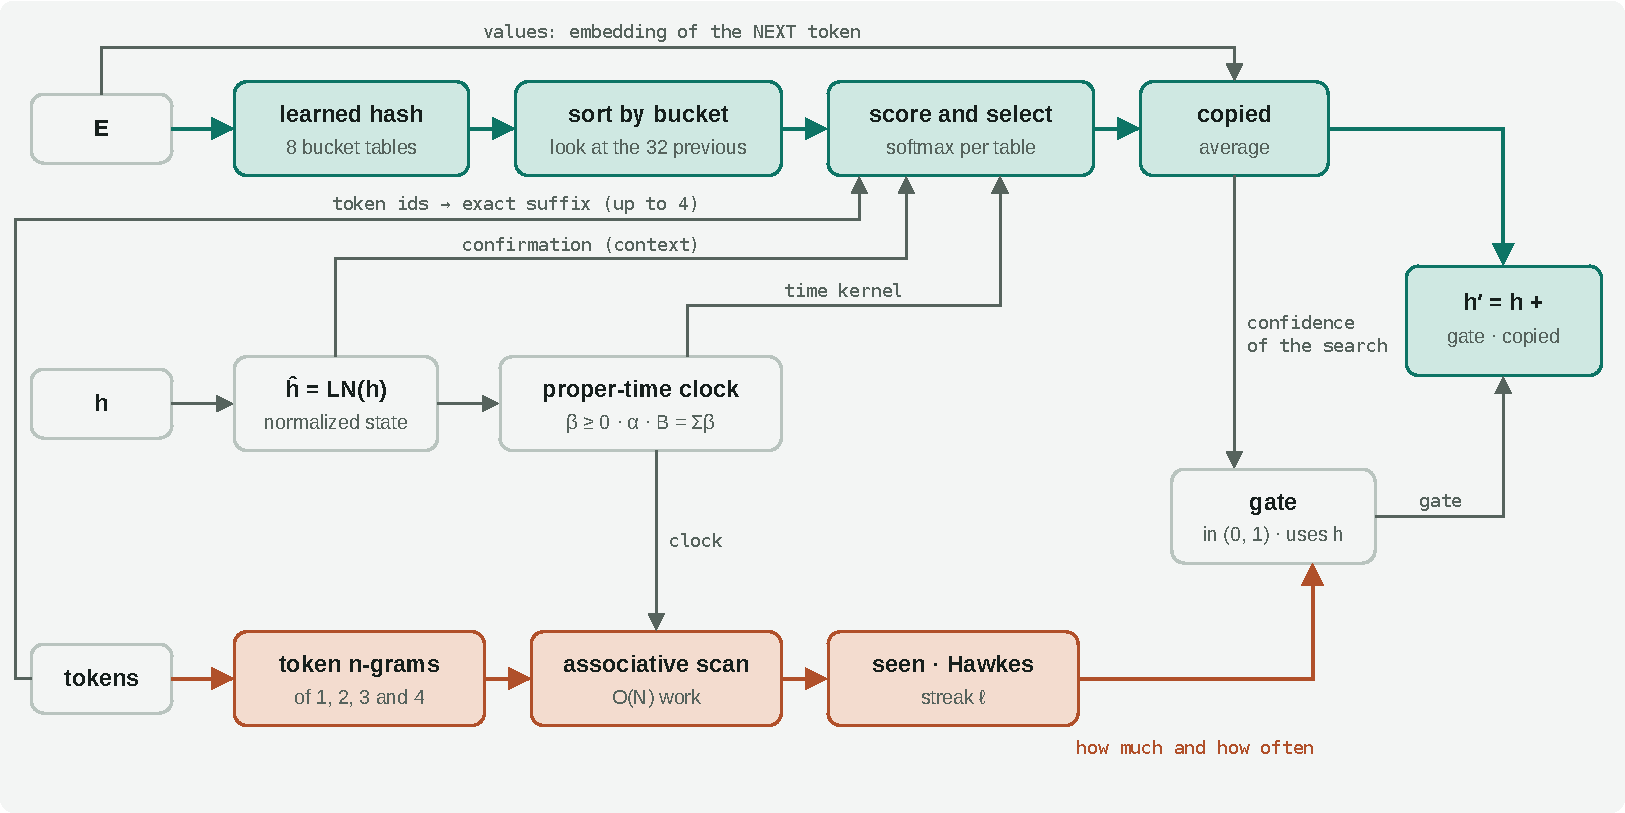
\includegraphics[width=0.78\linewidth]{capa_diagrama.pdf}
\caption{Inside an ASRN layer. Green: \emph{where to copy}---learned hash, sort by bucket, scores with a softmax per
table, and the average of the copied values (the embedding of the \emph{next} token). Orange: \emph{whether to
copy}---token $n$-grams and an associative scan give the repetition memory (seen flags, Hawkes intensity and the streak,
written $\ell$ in the diagram and $\rho$ in the text), read by the gate with the confidence of the search. The
proper-time clock, computed from the normalized state, feeds the time kernel of the scores and the scan.}
\label{fig:diagram}
\end{figure}

Tokens $x_t\in\{0,\dots,V-1\}$ are embedded as $E_t=\mathrm{Emb}[x_t]\in\mathbb{R}^d$. The model stacks causal
\emph{local blocks}, each a dense causal convolution over the current and $k-1=3$ previous positions followed by an MLP
of width $2d$,
\begin{equation}
h\leftarrow h+\GELU\!\big(\mathrm{Conv}^{\mathrm{causal}}_k(\LN_1 h)\big),\qquad
h\leftarrow h+W_2\,\GELU(W_1\LN_2 h),
\end{equation}
and inserts an ASRN layer after every second local block (after blocks $0,2,4,\dots$, except the last; a development
choice, see \nolinkurl{history/}). The output
reuses the embedding matrix, $p(x_{t+1}\mid x_{\le t})=\softmax(\mathrm{Emb}\,\LN_f h_t)$; there is no positional table,
so order enters through the convolutions and the clock. An ASRN layer maps the state $h$ to
\begin{equation}
\boxed{\;h'_t=h_t+g_t\,W_o\,c_t\;}
\label{eq:layer}
\end{equation}
where $c_t$ is what is \emph{copied} (Sec.~\ref{sec:search}) and $g_t\in(0,1)$ is the copy \emph{gate}
(Sec.~\ref{sec:gate}); Figure~\ref{fig:diagram} shows the data flow. Default sizes: $T=8$ tables of $b=14$ bits (four
of them also see the previous token), $C=32$ candidates, a 16-dimensional confirmation, suffixes up to 4 tokens and
$n$-grams of 1 to 4 tokens.

\subsection{Proper-time clock}
\label{sec:clock}
From the normalized state $\hat h_t=\LN(h_t)$ each layer computes two scalars per token:
\begin{equation}
\beta_t=\softplus(w_\beta^\top\hat h_t+b_\beta)\ge0,\qquad
\alpha_t=2\,\sigma(w_\alpha^\top\hat h_t+b_\alpha)\in(0,2),\qquad
B_t=\sum_{u\le t}\beta_u .
\label{eq:clock}
\end{equation}
$B_t$ is a monotone, data-dependent reparametrization of time: a token may advance the clock a lot (a topic change) or
almost nothing (inside a quotation), and $\alpha_s$ says how memorable occurrence $s$ is. Memory decays with the
continuous kernel
\begin{equation}
K_\kappa(t,s)=\alpha_s\,e^{-\kappa\,(B_t-B_s)},
\label{eq:kernel}
\end{equation}
an exponential kernel whose distance is proper time rather than token count. At initialization $\beta_t=\alpha_t=1$,
so the clock counts tokens.

\subsection{Where to copy: hashed sparse retrieval}
\label{sec:search}
Two small MLPs produce $T\cdot b$ hash coordinates per token; half of the tables also see the previous token:
\begin{equation}
\varphi_t=\big[f_{\mathrm{word}}(E_t)\,;\,f_{\mathrm{ctx}}([E_t;E_{t-1}])\big]\in\mathbb{R}^{Tb},\qquad
\kappa_\tau(t)=\sum_{j=0}^{b-1}2^j\,\mathbf{1}[\varphi_{t,\tau,j}>0].
\end{equation}
In table $\tau$, token $t$ considers only earlier tokens in its own bucket, at most the $C$ most recent:
$\Nset_\tau(t)=\{$the $C$ largest $s<t$ with $\kappa_\tau(s)=\kappa_\tau(t)\}$. These sets come from a stable sort of
positions by bucket followed by windows of $C$ queries against $2C$ keys, so the work per token is bounded and
causality holds by construction ($s<t$). Each candidate is scored by
\begin{equation}
\mathrm{score}_\tau(t,s)=
\underbrace{\frac{\langle\varphi_t,\varphi_s\rangle}{\sqrt{Tb}}}_{\text{hash similarity}}
+\underbrace{\frac{\langle W_q\hat h_t,W_k\hat h_s\rangle}{\sqrt{16}}}_{\text{confirmation}}
+\underbrace{w^{\mathrm{suf}}_{\ell(t,s)}}_{\text{exact suffix}}
+\underbrace{\log\alpha_s-\frac{\gamma_\tau}{C}\,(B_t-B_s)}_{\text{proper-time kernel}},
\label{eq:score}
\end{equation}
where $\ell(t,s)\in\{0,\dots,4\}$ is the length of the exact common suffix ($x_{t-1}=x_{s-1}$, $x_{t-2}=x_{s-2}$,
\dots) and $\gamma_\tau$ is a learned per-table time scale. The last term is the logarithm of
kernel~\eqref{eq:kernel}: after the softmax it is a \emph{normalized} proper-time kernel. The layer copies the token
that came \emph{after} each match:
\begin{equation}
a_\tau(t,s)=\softmax_{s\in\Nset_\tau(t)}\mathrm{score}_\tau(t,s),\qquad
o_\tau(t)=\sum_{s\in\Nset_\tau(t)}a_\tau(t,s)\,W_vE_{s+1},\qquad
c_t=\frac{\sum_\tau o_\tau(t)}{\max(1,n_t)},
\end{equation}
with $n_t$ the number of tables in which $t$ has at least one candidate ($o_\tau(t)=0$ otherwise).

\subsection{Whether to copy: Hawkes intensity and repetition streak}
\label{sec:repetition}
To decide whether the text is currently quoting, for the $n$-gram ending at $t$, $G_n(t)=(x_{t-n+1},\dots,x_t)$,
$n=1,\dots,4$, the layer computes
\begin{align}
v_n(t)&=\mathbf{1}\big[\exists\,s<t:\,G_n(s)=G_n(t)\big] &&\text{(seen)}\\
\lambda_n(t)&=\sum_{s<t,\;G_n(s)=G_n(t)}\alpha_s\,e^{-\kappa_n(B_t-B_s)} &&\text{(Hawkes intensity)}\label{eq:hawkes}\\
\rho_t&=v_4(t)\,\big(e^{-\kappa_r\beta_t}\,\rho_{t-1}+1\big),\quad\rho_0=0 &&\text{(repetition streak)}\label{eq:streak}
\end{align}
Equation~\eqref{eq:hawkes} is the intensity of a self-exciting point process~\cite{hawkes1971spectra} whose events are
the past occurrences of the same $n$-gram, with the \emph{unnormalized} kernel~\eqref{eq:kernel} as excitation. The
streak $\rho_t$ measures the length of the quotation in progress. The rates $\kappa_n,\kappa_r>0$ are learned, starting
from $\kappa_n=1/(C\,4^{\,n-1})$ and $\kappa_r=1/(8C)$: short $n$-grams forget quickly, long ones remember longer.

\subsection{The gate and its non-monotone response}
\label{sec:gate}
\begin{equation}
g_t=\sigma\Big(w_g^\top h_t+w_{\mathrm{conf}}^\top\mathrm{conf}_t+b
+\sum_{n=1}^{4}w_n\,v_n(t)+\sum_{n=1}^{4}u_n\log\!\big(1+\lambda_n(t)\big)+f(\rho_t)\Big),
\end{equation}
where $\mathrm{conf}_t$ are four retrieval-confidence signals (fraction of tables with candidates, best score, peak
attention, fraction of context tables with candidates). The streak response $f$ is piecewise linear on 16 nodes equally
spaced in $\log(1+\rho)$ up to $\rho=256$ and constant beyond, parametrized by \emph{increments}:
\begin{equation}
z=\frac{\log(1+\rho)}{\Delta},\;\;\Delta=\frac{\log 257}{15},\;\;i=\lfloor z\rfloor,\qquad
f(\rho)=U_i+(z-i)(U_{i+1}-U_i),\qquad U_i=\sum_{j\le i}\delta_j .
\label{eq:response}
\end{equation}
A monotone response (e.g.\ $u\log(1+\rho)$) cannot express ``continue up to the usual length of a quotation, then
stop''; \eqref{eq:response} can, and since nodes that never see data receive zero gradient, the curve extrapolates
\emph{flatly} from the last observed node. The motivation is \emph{state aliasing}: a gate that only sees saturating
signals (seen flags, suffixes up to 4 tokens) cannot tell a quotation of 5 tokens from one of 50.

\subsection{One associative scan for every recurrence}
\label{sec:scan}
Seen flags, Hawkes intensities and the streak are linear recurrences $S_i=a_iS_{i-1}+b_i$ with $a_i\in[0,1]$. Affine
maps compose associatively, $(a_1,b_1)\circ(a_2,b_2)=(a_1a_2,\,a_2b_1+b_2)$, so all positions are solved in parallel
by a scan~\cite{blelloch1990prefix,martin2018parallelizing}: $O(N)$ work, $O(\log N)$ depth, and only products in
$[0,1]$ and sums (stable in fp32 and bf16). Setting $a_i=0$ restarts the recurrence, so all segments are scanned at
once. The Hawkes intensity reuses the sort of the seen flags: in the order sorted by $n$-gram key, the previous
occurrence of the same $n$-gram is the previous element and
\begin{equation}
S_i=a_i\,(S_{i-1}+\alpha_{i-1}),\qquad
a_i=\begin{cases}e^{-\kappa_n(B_i-B_{i-1})}&\text{same }n\text{-gram as }i-1\\0&\text{otherwise.}\end{cases}
\label{eq:scan}
\end{equation}

\paragraph{Initialization, complexity and generation.} $w_\alpha$, $\gamma$, $w_n$, $u_n$, $\delta_j$,
$w^{\mathrm{suf}}$, $w_{\mathrm{conf}}$ and $W_q$ start at zero and $\beta_t=\alpha_t=1$, so a new layer computes what
the simpler layer without clock, Hawkes and streak computed. Per token and table, ASRN scores one window of $2C$ keys;
only the sort by bucket grows with $N$ ($O(N\log N)$ with a comparison sort, a radix sort with fixed passes on the GPU),
and saved memory is $O(N)$. Counted on CPU, a layer with $d=512$ costs 5.19 and 5.13 MFLOP per token at 1{,}024 and
16{,}384 tokens, against 9.44 and 56.62 for attention. In generation each table keeps, per bucket, a ring with the $C$
most recent positions, which are exactly the keys a new token attends to, and each $n$-gram key carries the clock $B_u$
of its last occurrence and $A=\lambda_n(u)+\alpha_u$, so that $\lambda_n(t)=e^{-\kappa_n(B_t-B_u)}A$ and then
$A\leftarrow\lambda_n(t)+\alpha_t$, $B_u\leftarrow B_t$ (the recurrence~\eqref{eq:scan} carried one step at a time); the
streak is one number. Each new token therefore costs $O(1)$ time, independent of the context, while the memory still
grows with the text (the cached features of every position, plus fixed rings of 17\,MiB per layer and sequence at the
default sizes). By default the candidates are restricted to positions whose continuation lies inside the prompt
(\emph{prompt-only copy memory}), so the model cannot get trapped copying its own output, and a
\emph{quotation-preserving temperature} rescales the sampled distribution so that the tokens that would continue an
already-seen 4-gram keep the model's own probability at $T=1$.

\subsection{Numerical protections (ASRN 1.0)}
\label{sec:protections}
Release 1.0 keeps the v89 layer (\nolinkurl{asrn/nucleo.py}) and adds a protected layer with the same parameters
(\nolinkurl{asrn/estable.py}), used by default. It reproduces v89 up to rounding in the normal regime
($1.3\cdot10^{-7}$ in the logits) and closes failure modes of v89 found by measurement (A100, TF32 off):
\begin{itemize}
\item \textbf{Exact masking.} v89 gives invalid keys a finite score $-10^9$; if every valid score falls far below it,
  the softmax mass moves to invalid keys, among them the query itself, whose value is the next token. With
  $\gamma=10^9$ the future changed the past by $1.6\cdot10^{-2}$; normalizing over valid keys only makes it 0.
\item \textbf{64-bit clock.} An fp32 clock knows the increment $B_t-B_{t-1}$ only to a median 2.2\% at $2^{20}$ tokens
  and stops on 16\% of the steps at $2^{24}$, and v89's time term $(\log\alpha_s+rB_s)-rB_t$ cancels: shifting the clock
  by $10^9$ changes the output by $8.8\cdot10^{-2}$. The stable layer accumulates $B$ in fp64, passes it to the kernel
  in two fp32 parts and subtracts them before multiplying by the rate: shifts of $10^6$, $1.6\cdot10^7$ and $10^9$ all
  change the output by $5.5\cdot10^{-8}$, a constant rounding difference. Its clock projection runs in true fp32:
  switching TF32 on moves the clock over 65{,}536 tokens by up to 1.98 units in v89 and by $1.16\cdot10^{-10}$ in the
  stable layer.
\item \textbf{Bounds}: $\beta\le10^4$, $\log\alpha\ge-30$, and the best-score gate signal clipped to $\pm10^4$.
\end{itemize}
They cost +7.5\% time and +5.2\% memory for one layer at 262{,}144 tokens (Table~\ref{tab:layer}). A second group of
protections changes the function and is off by default; it had no measurable cost or effect in the ablation.

\section{Experiments}
\label{sec:experiments}

\paragraph{Setup.} All GPU numbers come from one execution of \nolinkurl{benchmarks/asrn_colab.ipynb} on 17 October
2026 on one NVIDIA A100-SXM4-80GB in Google Colab (PyTorch 2.14.1, CUDA 13.0, bf16 autocast, code fingerprint
\texttt{5164e1f32513}); raw results are in \nolinkurl{results/banco_a100/}. ASRN is the stable layer of release 1.0. The
baselines have the same width and nearly the same number of parameters: \emph{Transformer++}, our implementation of the
Llama recipe~\cite{touvron2023llama} (RMSNorm, SwiGLU, RoPE~\cite{su2024roformer}; the name follows~\cite{gu2023mamba})
with FlashAttention-2 through PyTorch SDPA and its other operations unfused; \emph{Mamba-2}, the original block of
\texttt{mamba\_ssm} 2.3.2 without \texttt{causal-conv1d} (its unfused path, so ASRN's speed ratios against it are upper
bounds); and \emph{RWKV-7}, the original \texttt{RWKV7Model} of flash-linear-attention 0.5.2~\cite{yang2024fla}. All use
the same training loop (AdamW, warm-up and cosine decay, clipping at 1, bf16, the same batches within a seed). For each
model and task, the better of two learning rates ($10^{-3}$, $3\cdot10^{-3}$) on seed 0 by the metric at the training
length (ties to the lower) is repeated with seeds 1 and 2; we report mean $\pm$ sd over 3 seeds. The rate is selected on
the reported evaluation, and the comparison is at equal data, not equal compute. Only the training throughput of ASRN
and the Transformer++ was also measured compiled.

\subsection{The bottleneck: one layer from 1k to 262k tokens}
\label{sec:layer}

\begin{figure}[t]
\centering
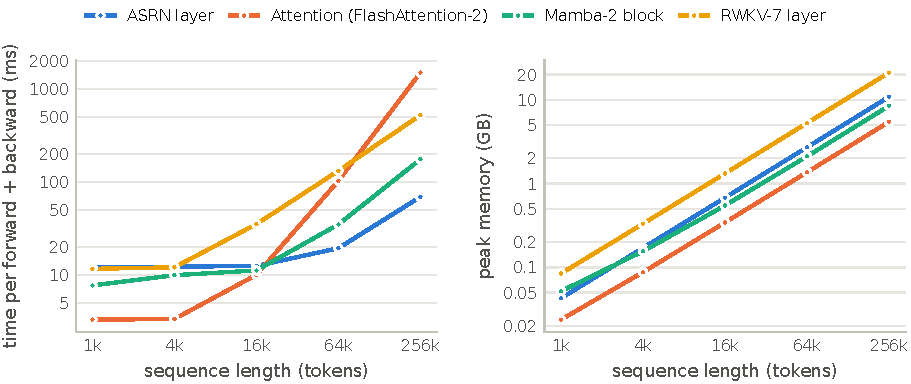
\includegraphics[width=0.94\linewidth]{capa.pdf}
\caption{One layer, forward + backward, $d=512$, batch 1, bf16, uncompiled. Left: time; right: peak memory; both axes
logarithmic. The ASRN layer is the stable layer of release 1.0; attention is FlashAttention-2 with its RMSNorm; the
Mamba-2 unit is its whole block (2.6$\times$ the parameters of the ASRN layer); the RWKV-7 layer is the first layer of
a two-layer model.}
\label{fig:layer}
\end{figure}

\begin{table}[t]
\centering\small
\begin{tabular}{lrrrrrrr}
\toprule
& \multicolumn{3}{c}{time (ms)} & \multicolumn{2}{c}{peak memory (GB)} & KiB/token & local \\
\cmidrule(lr){2-4}\cmidrule(lr){5-6}
Layer & 1{,}024 & 65{,}536 & 262{,}144 & 65{,}536 & 262{,}144 & at 262k & exponent\\
\midrule
ASRN 1.0 (stable layer) & 12.1 & \textbf{19.3} & \textbf{68.7} & 2.71 & 10.85 & 40 & 0.92\\
ASRN v89 (no protections) & 12.0 & 18.0 & 64.0 & 2.58 & 10.31 & 38 & 0.91\\
Attention (FlashAttention-2) & \textbf{3.3} & 102.4 & 1{,}486.0 & \textbf{1.37} & \textbf{5.46} & \textbf{20} & 1.93\\
Mamba-2 block & 7.7 & 34.8 & 174.3 & 2.12 & 8.45 & 31 & 1.16\\
RWKV-7 layer & 11.6 & 131.1 & 519.4 & 5.28 & 21.10 & 79 & 0.99\\
\bottomrule
\end{tabular}
\caption{One layer (the setting of Fig.~\ref{fig:layer}). Local exponent: log-log slope of time between 65{,}536 and
262{,}144 tokens (1 = linear, 2 = quadratic); the memory exponent is 1.00 for all. Bold: best of the four units.}
\label{tab:layer}
\end{table}

Attention has linear memory but quadratic time (Fig.~\ref{fig:layer}, Table~\ref{tab:layer}). ASRN's time has a floor
of about 12\,ms up to 16k tokens (most likely kernel-launch overhead; not profiled) and then grows almost linearly.
Below 16k tokens ASRN is among the slowest units (attention is 3.7$\times$ faster at 1k--4k tokens; RWKV-7 ties).
Interpolating linearly, ASRN overtakes attention at $\approx$17.8k tokens and the Mamba-2 block at $\approx$20.2k
(RWKV-7 at $\approx$4.2k); at 262{,}144 tokens it is 21.6$\times$ faster than attention, 2.5$\times$ faster than the
Mamba-2 block (a different, unfused unit; with whole models the ratio is 1.4--1.5) and 7.6$\times$ faster than RWKV-7.
Its memory is about 40\,KiB per token, 2.0$\times$ attention (RWKV-7 needs 1.9$\times$ ASRN's).

\subsection{Training throughput and generation}
\label{sec:throughput}

\begin{figure}[t]
\centering
\begin{minipage}[c]{0.54\linewidth}
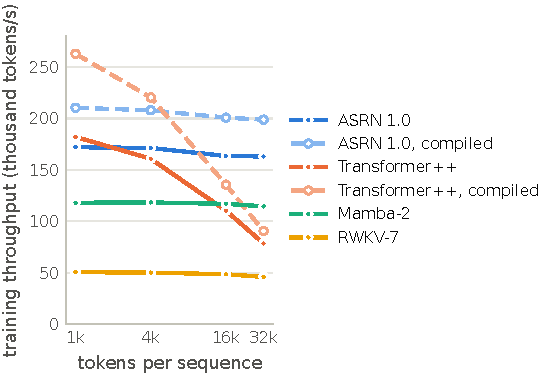
\includegraphics[width=\linewidth]{modelo.pdf}
\end{minipage}\hfill
\begin{minipage}[c]{0.43\linewidth}
\caption{Training throughput of $\approx$50M-parameter models (vocabulary 32{,}768, $d=512$) with 32{,}768 tokens per
step (batch $\times$ length), bf16. Solid: uncompiled. Dashed, open markers: ASRN compiled by parts and the
Transformer++ with \texttt{torch.compile}; Mamba-2 and RWKV-7 were not compiled.}
\label{fig:throughput}
\end{minipage}
\end{figure}

With the tokens per step fixed, uncompiled, ASRN trains at 172{,}065, 171{,}275, 163{,}503 and 163{,}023 tokens/s with
1k, 4k, 16k and 32k tokens per sequence ($-5.3\%$; Fig.~\ref{fig:throughput}) and the Transformer++ at 182{,}116 down to
78{,}400 ($-57\%$): the Transformer++ is 6\% faster at 1{,}024 tokens, and ASRN 1.07, 1.48 and 2.08$\times$ faster at
4k, 16k and 32k (crossover $\approx$2.4k). ASRN is 1.40--1.46$\times$ faster than the unfused Mamba-2 and
3.38--3.55$\times$ faster than RWKV-7. Compiled by parts, ASRN trains at 210{,}413 to 198{,}826 tokens/s
(1.21--1.23$\times$ its uncompiled speed), and \texttt{torch.compile} speeds the Transformer++ up by 1.44$\times$ at
1{,}024 tokens (262{,}909) and 1.15$\times$ at 32{,}768 (90{,}540): with both compiled the crossover moves to
$\approx$5.4k tokens (Transformer++ 1.25$\times$ faster at 1{,}024, ASRN 2.20$\times$ faster at 32{,}768). ASRN's peak
memory (23.5\,GB) is 8\%, 11\% and 23\% below that of the Transformer++, Mamba-2 and RWKV-7.

\paragraph{Generation.} With batch 1 and the earlier $O(t)$ writer, ASRN generated slowest: about 43\,ms per new token
(mean 43.05 over contexts of 1k--64k tokens), against 14.75 for the Transformer++, 24.84 for Mamba-2 and 36.51 for
RWKV-7. The $O(t)$ term was hidden under a per-token overhead (fitted slope 3.0\,ns per context token, 95\% CI $-25$ to
31), most likely kernel launches (not profiled). The prefix pass over 65{,}536 tokens takes 0.140\,s for ASRN, 0.387\,s
for the Transformer++ and 0.139\,s for Mamba-2 (RWKV-7: 110.9--130.9\,s at every length, mostly kernel compilation or
autotuning). The $O(1)$ writer of release 1.0 gives the same outputs (largest difference $2.2\cdot10^{-7}$ against the
whole-text forward pass) but has not yet been measured on the A100. On CPU (4 threads, a 0.70M-parameter model with 2
ASRN layers, batch 1; \nolinkurl{results/escritura_cpu/}) it stays at 9.5--12.5\,ms per new token from 512 to 131{,}072
tokens of context (slope $-19$\,ns per context token, 95\% CI $-42$ to 3), while the $O(t)$ writer grows from 15.8 to
91.7\,ms (583\,ns, CI 537 to 629): 1.27$\times$ faster at 512 tokens and 9.7$\times$ at 131{,}072.

\subsection{Long-range copying and associative recall}
\label{sec:copy}

\begin{figure}[t]
\centering
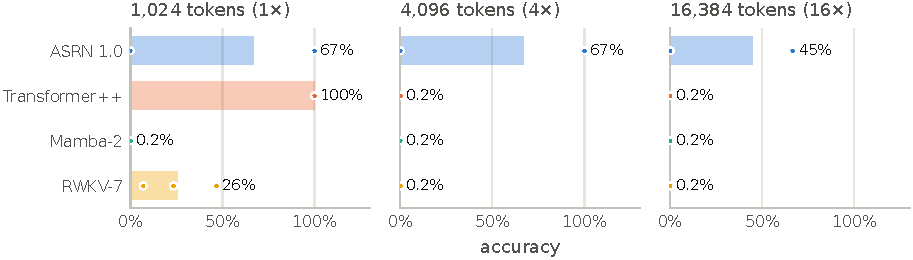
\includegraphics[width=0.92\linewidth]{copia.pdf}\\[3pt]
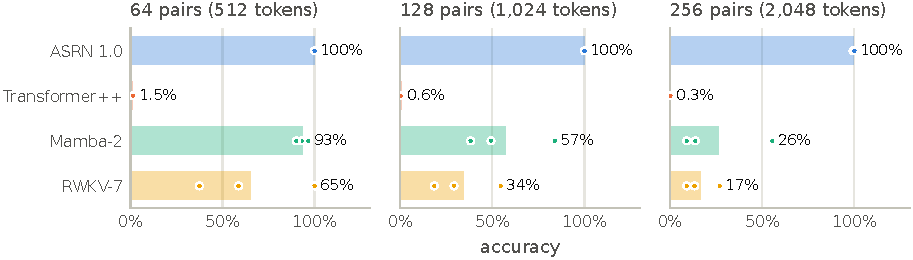
\includegraphics[width=0.92\linewidth]{mqar.pdf}
\caption{Top: copy accuracy at 1$\times$, 4$\times$ and 16$\times$ the training length; a training sequence is 512
random tokens (vocabulary 512) followed by their exact repetition, so its second half requires copying from 512 tokens
back. Bottom: MQAR~\cite{arora2023zoology} accuracy on the queried values, trained with 64 key--value pairs in 512
tokens (vocabulary 8{,}192) and evaluated with 64, 128 and 256 pairs at 512, 1{,}024 and 2{,}048 tokens. Bars and
printed values: mean of 3 seeds; dots: each seed. ASRN's copy mean hides two seeds that learned and one that stayed on
the initial plateau (dot near 0\%). Copy chance: 0.2\%.}
\label{fig:copy}
\end{figure}

\begin{table}[t]
\centering\small
\setlength{\tabcolsep}{3pt}
\begin{tabular}{llrrrl}
\toprule
\textbf{Copy} & lr & 1{,}024 (1$\times$) & 4{,}096 (4$\times$) & 16{,}384 (16$\times$) & loss $<1$ at step\\
\midrule
ASRN, seeds 0, 2 (learned) & $10^{-3}$ & 100.00, 100.00 & 99.99, 99.98 & 66.83, 66.49 & 1{,}000, 1{,}000\\
ASRN, seed 1 (plateau) & & 0.10 & 0.15 & 0.18 & never\\
ASRN, mean $\pm$ sd (3 seeds) & & $66.70\pm57.68$ & $66.71\pm57.64$ & $44.50\pm38.38$ & \\
Transformer++ & $10^{-3}$ & $100.00\pm0.00$ & $0.20\pm0.03$ & $0.22\pm0.01$ & 200 (all seeds)\\
Mamba-2 & $3\cdot10^{-3}$ & $0.19\pm0.07$ & $0.19\pm0.02$ & $0.21\pm0.01$ & never\\
RWKV-7 & $10^{-3}$ & $25.77\pm19.98$ & $0.25\pm0.02$ & $0.22\pm0.01$ & never\\
\midrule
\textbf{MQAR} & lr & 512 (64 pairs) & 1{,}024 (128) & 2{,}048 (256) & 2{,}048, per seed\\
\midrule
ASRN & $3\cdot10^{-3}$ & $\mathbf{99.99\pm0.02}$ & $\mathbf{99.99\pm0.01}$ & $\mathbf{99.75\pm0.43}$ &
100.00 / 99.25 / 99.99\\
Transformer++ & $3\cdot10^{-3}$ & $1.50\pm0.18$ & $0.56\pm0.18$ & $0.34\pm0.12$ & 0.31 / 0.46 / 0.24\\
Mamba-2 & $3\cdot10^{-3}$ & $93.20\pm3.27$ & $57.17\pm23.85$ & $26.09\pm25.55$ & 9.11 / 55.48 / 13.68\\
RWKV-7 & $10^{-3}$ & $65.43\pm31.76$ & $34.16\pm18.51$ & $16.51\pm9.34$ & 9.14 / 13.38 / 27.01\\
paired $p$, ASRN vs Mamba-2 & & $p=0.070$ & $p=0.090$ & $p=0.039$ & \\
paired $p$, ASRN vs RWKV-7 & & $p=0.20$ & $p=0.025$ & $p=0.0041$ & \\
\bottomrule
\end{tabular}
\caption{Copy (2.5--2.9M parameters) and MQAR (4.4--4.9M) accuracy (\%), 2{,}000 training steps, mean $\pm$ sd over
3 seeds (per-seed values in seed order 0 / 1 / 2; paired $t$-tests over seeds). ASRN left the initial copy
plateau in 2 of 3 seeds; seed 1 stayed on it for all 2{,}000 steps (final loss 6.232 $\approx\ln 511$). In the previous
A100 run (Section~\ref{sec:replication}) all 3 seeds learned the copy ($99.87\pm0.18$\% at 4$\times$).}
\label{tab:copy}
\end{table}

\paragraph{Copy.} When ASRN leaves the initial plateau it copies without error at the training length and nearly
without error at 4$\times$ (Fig.~\ref{fig:copy}, top; Table~\ref{tab:copy}). Leaving it within 2{,}000 steps at
$10^{-3}$ is not guaranteed (5 of the 6 base runs of the two A100 runs did), but this is optimization rather than
capacity: with $3\cdot10^{-3}$ seed 0 left it by step 400 and reached 100\%, 99.99\% and 97.62\% (both rates tied at
100\% at the training length, so the lower was selected). The Transformer++ learns the task at least 4$\times$ earlier
than ASRN's learned seeds but falls to chance beyond its training length, which these data cannot attribute to RoPE at
unseen distances~\cite{press2022alibi} rather than to a head that learned a fixed offset of 511. Mamba-2 and RWKV-7 did
not learn within this budget, which does not show that they cannot copy: ASRN itself sat on the same plateau for about
800 steps.

\paragraph{MQAR.} ASRN keeps its recall as the number of pairs grows (Fig.~\ref{fig:copy}, bottom), at least 99.25\% in
every seed; it selected $3\cdot10^{-3}$ by a near tie on seed 0 (100.00\% against 99.97\%). Mamba-2 falls from 93.2\%
to 26.1\%, the decline expected of a fixed-size state~\cite{arora2023zoology}, confounded with length extrapolation and
with incomplete convergence (final loss 0.33, 0.16 and 0.49); two RWKV-7 seeds did not converge (final loss 3.40 and
2.05). The Transformer++ did not learn MQAR with either rate (final loss 7.43--8.21, near $\ln 4096=8.32$), a failure of
this budget or protocol rather than of attention~\cite{arora2023zoology}. The rivals' results are not stable across runs
(Section~\ref{sec:replication}); this MQAR, with unique keys followed by their values, is at ceiling for ASRN.

\subsection{Language modeling}
\label{sec:lm}

\begin{figure}[t]
\centering
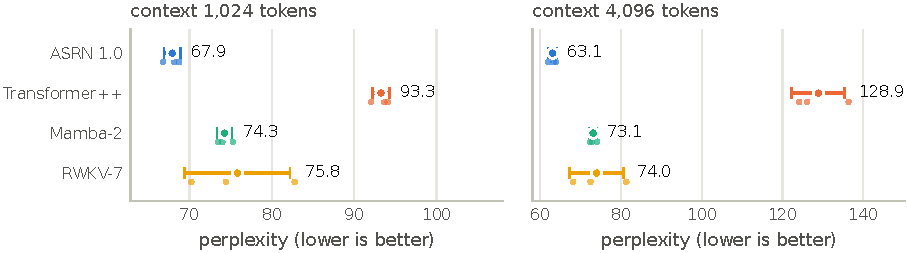
\includegraphics[width=0.94\linewidth]{texto.pdf}
\caption{WikiText-103 validation perplexity (lower is better) with 1{,}024 and 4{,}096 tokens of context, after
1{,}220 steps of 16 sequences of 1{,}024 tokens ($\approx$45M parameters, $d=512$). Large dot and bar: mean $\pm$ 1
sd of 3 seeds (mean printed); small dots: each seed.}
\label{fig:text}
\end{figure}

\begin{table}[t]
\centering\small
\begin{tabular}{lrlrrrl}
\toprule
& & & \multicolumn{2}{c}{perplexity} & & paired $p$ vs ASRN\\
\cmidrule(lr){4-5}
Model & Params & lr & context 1{,}024 & context 4{,}096 & 4k vs 1k & (1{,}024 / 4{,}096)\\
\midrule
ASRN 1.0 & 45.1M & $3\cdot10^{-3}$ & $\mathbf{67.91\pm1.00}$ & $\mathbf{63.08\pm0.97}$ & $-7.1\%$ & ---\\
Transformer++ & 44.4M & $10^{-3}$ & $93.27\pm1.07$ & $128.87\pm6.56$ & $+38.2\%$ & 0.002 / 0.003\\
Mamba-2 & 44.7M & $3\cdot10^{-3}$ & $74.25\pm0.92$ & $73.09\pm0.88$ & $-1.6\%$ & 0.008 / 0.003\\
RWKV-7 & 46.3M & $3\cdot10^{-3}$ & $75.81\pm6.39$ & $73.96\pm6.71$ & $-2.4\%$ & 0.13 / 0.084\\
\bottomrule
\end{tabular}
\caption{WikiText-103~\cite{merity2016pointer} (GPT-2 tokenizer), mean $\pm$ sd over 3 seeds; paired $t$-test over
seeds. The difference with RWKV-7 is not significant.}
\label{tab:text}
\end{table}

At equal data and size (Fig.~\ref{fig:text}, Table~\ref{tab:text}), ASRN is best in every seed (66.81--68.76). Its
advantage over the Transformer++ and Mamba-2 is significant at both context lengths; over RWKV-7 it is not: RWKV-7
varies strongly across seeds (70.24--82.78) and trails ASRN in all three, by 6.26, 3.43 and 14.02. The caveats weigh
heavily: the models are far from convergence (about 0.44 training positions per parameter); the rates sit at the edges
of the grid (with the same $10^{-3}$ on seed 0 the order was Mamba-2 86.09, ASRN 89.55, Transformer++ 94.07); and
WikiText-103 rewards copying, which ASRN's exact matching favours. As development history, the fifth development run
(\nolinkurl{history/}), with another protocol and a \emph{reimplemented} RWKV-7, found RWKV-7 clearly best
($47.87\pm0.15$ against $57.02\pm0.32$ for the v89 ASRN recipe). No general claim that ASRN beats RWKV-7 on text is
supported.

\subsection{Ablation: retrieval and regulation on pure-copy tasks}
\label{sec:ablation}

\begin{table}[t]
\centering\small
\setlength{\tabcolsep}{3pt}
\begin{tabular}{llccrr}
\toprule
& & \multicolumn{2}{c}{copy: seeds that learned} & copy 4$\times$, & MQAR 2{,}048,\\
\cmidrule(lr){3-4}
Variant & Change & this run & both runs & worst learned (\%) & mean (\%)\\
\midrule
\texttt{estable\_A} (base) & --- & 2 of 3 & 5 of 6 & 99.98 & 99.75\\
\texttt{estable\_AB} & + group B & 2 of 3 & 5 of 6 & 99.89 & 99.29\\
\texttt{sin\_puerta} & gate fixed at 1 & 2 of 3 & 4 of 6 & 99.98 & 99.94\\
\texttt{puerta\_sin\_senales} & gate sees only $h$ & 3 of 3 & 6 of 6 & 99.98 & 99.50\\
\texttt{sin\_reloj} & $\beta=\alpha=1$, $\gamma=0$ & 2 of 3 & 4 of 6 & 99.98 & 99.95\\
\texttt{sin\_hawkes\_racha} & Hawkes, streak frozen & 3 of 3 & 6 of 6 & 99.98 & 99.53\\
\texttt{sin\_sufijo} & suffix weight frozen & 2 of 3 & 4 of 6 & 39.77 & 99.69\\
\texttt{sin\_confirmacion} & confirmation frozen & 3 of 3 & 6 of 6 & 99.93 & 99.88\\
\texttt{dos\_tablas} & 1 + 1 tables & 1 of 3 & 2 of 6 & 99.67 & 98.99\\
\texttt{solo\_local} & no ASRN layer & 0 of 3 & 0 of 6 & --- & 0.31\\
\texttt{mezcla\_lse} & log-normalizer mixing & 1 of 3 & 4 of 6 & 92.67 & 2.61\\
\bottomrule
\end{tabular}
\caption{Ablation: the stable layer with one component removed, 3 seeds, at ASRN's selected rates; the base row is the
quality run of Section~\ref{sec:copy}. ``Both runs'' adds the 3 seeds of the previous A100 run. Frozen components stay
at their neutral initial value, so those variants compute the base function at step 0, on the same batches;
\texttt{dos\_tablas} uses 1 + 1 tables instead of 4 + 4.}
\label{tab:ablation}
\end{table}

Copy is bimodal (a run either leaves the initial plateau or stays at chance), so Table~\ref{tab:ablation} reports
learned runs separately. \textbf{The ASRN layer is what solves both tasks}: without
it (\texttt{solo\_local}, a receptive field of 13 tokens) both stay at chance in every seed of both A100 runs.
\textbf{On these tasks the retrieval core is sufficient and the regulation mechanisms are non-intrusive}: the learned
copy runs of the base and the regulation variants copy at 4$\times$ with at least 99.89\%, and their MQAR means stay
between 99.29\% and 99.95\%. \textbf{Three seeds cannot show that removing the gate, the clock or the suffix harms
learning}: the base itself stayed on the copy plateau with seed 1, as did five variants (across both runs, 5 of 6 for
the base against 4 of 6 without the gate, the clock or the suffix; Fisher $p=0.50$, one-sided). Fewer tables (2 of 6;
$p=0.12$) and the \texttt{sin\_sufijo} run that gave 87.02\% at 1$\times$ but 39.77\% at 4$\times$ are suggestive only.
Log-normalizer mixing, which left the copy plateau first in all 3 seeds of the previous run, did so in 1 of 3 here,
does not learn MQAR and costs +62\% per copy run; it stays outside 1.0. Without the gate, its signals, Hawkes and
streak, or the clock, a copy run takes 17\%, 15\%, 8\% and 6\% less time; what these mechanisms buy is measured in
open-ended generation.

\subsection{Learning when to stop copying}
\label{sec:quote}

% Body of Section "Learning when to stop copying" (\input from ASRN_Calvario_2026_en.tex).
% Sources: results/citas (CPU, the primary run), results/citas_a100 (its A100 replication),
% docs/TECHNICAL_REPORT.md (Section 7.2). Script: benchmarks/experimento_citas.py.

Copy and MQAR cannot exercise the regulation mechanisms: every evaluated position requires a copy, so retrieval is all
they need, and there the gate, the clock and the Hawkes and streak signals were shown only to be non-intrusive (with
them ASRN copies at 4$\times$ with 99.99\% and 99.98\% in the 2 of 3 seeds that learned and reaches 99.75\% on MQAR
with 4$\times$ the pairs; Section~\ref{sec:ablation}). Their job, deciding whether to copy and when to stop, matters in
free generation, so their active role is tested there, on text whose quotations have a bounded length.

\paragraph{Setup.} The text is random tokens ($V=64$) in which, with probability 0.04 per position, a span of the last
200 tokens of uniform length 6--12 is quoted; in the real text 15.6\% of the tokens are quoted, and runs of
already-seen 4-grams rarely exceed 9 tokens (0.9\% do; the longest is 10). Five models are trained with the same seed,
data and recipe ($d=64$, two local blocks and one ASRN layer, $L=256$, batch 16, learning rate $3\cdot10^{-3}$, 6{,}000
steps on fresh text): the full 1.0 layer; the layer without the Hawkes and streak signals (frozen at their neutral
values); a gate that sees only the hidden state; no gate (fixed at 1); and no clock ($\beta=\alpha=1$, $\gamma=0$). Each
writes 128 tokens after 128-token prompts of 64 validation texts ($T=0.8$ with top-$k=40$ by default, and $T=1$; with
and without prompt-only copy memory). We measure the fraction of written tokens that close an already-seen
4-gram (\emph{quoted}) and the lengths of the runs of such tokens (\emph{streaks}), pooled over seeds 0, 1 and 2. The
primary run is on CPU (\nolinkurl{results/citas/}); the A100 benchmark repeated it (\nolinkurl{results/citas_a100/}).

\begin{figure}[t]
\centering
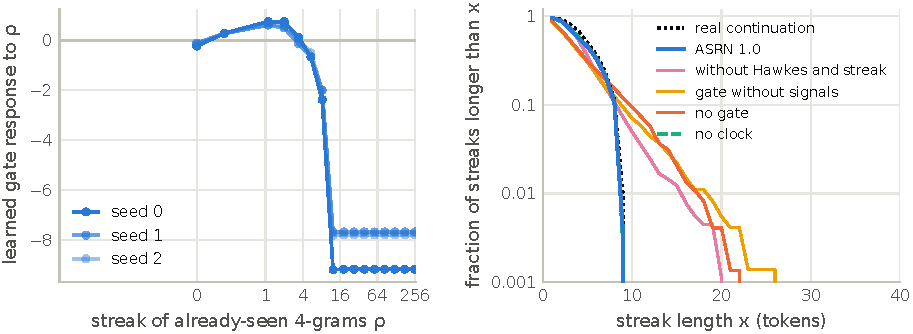
\includegraphics[width=0.94\linewidth]{citas.pdf}
\caption{Bounded-quotation experiment, CPU run. Left: the learned response $f(\rho)$ of the gate of the full layer to
the repetition streak $\rho$, three seeds (symmetric-log axis; nodes equally spaced in $\log(1+\rho)$ up to 256). Right:
fraction of the written streaks longer than $x$ tokens, pooled over the three seeds, with the default sampling
($T=0.8$, top-$k=40$, prompt-only copy memory on); the curve without the clock nearly coincides with the full layer's.}
\label{fig:quote}
\end{figure}

\begin{table}[t]
\centering\small
\setlength{\tabcolsep}{3.3pt}
\begin{tabular}{lrrlrlrl}
\toprule
& \multicolumn{5}{c}{CPU (primary run)} & \multicolumn{2}{c}{A100 replication}\\
\cmidrule(lr){2-6}\cmidrule(lr){7-8}
Text & quoted & mean & max (per seed) & $>9$ & val.\ loss & $>9$ & max (per seed)\\
\midrule
Real continuation & 15.6\% & 5.60 & 10 & 0.9\% & --- & 0.9\% & 10\\
\textbf{ASRN 1.0 (full layer)} & \textbf{20.9\%} & \textbf{5.24} & \textbf{10} (9/10/10) & \textbf{0.3\%} &
3.7027--3.7056 & \textbf{0.3\%} & \textbf{10} (9/10/10)\\
without Hawkes and streak & 19.0\% & 5.22 & 21 (21/20/20) & 7.2\% & 3.7070--3.7079 & 7.9\% & 19 (17/15/19)\\
gate without signals & 13.9\% & 4.69 & 27 (17/23/27) & 9.3\% & 3.7290--3.7586 & 9.2\% & 39 (24/21/39)\\
no gate & 14.7\% & 4.91 & 23 (19/21/23) & 11.8\% & 3.7320--3.7396 & 12.0\% & 21 (21/20/20)\\
no clock & 20.2\% & 5.25 & 10 (10/10/9) & 0.2\% & 3.7042--3.7053 & 0.4\% & 10 (9/10/9)\\
\bottomrule
\end{tabular}
\caption{Writing with the default sampling, seeds 0--2 pooled. \emph{Quoted}: fraction of written tokens that close an
already-seen 4-gram; \emph{mean}, \emph{max}: streak length; $>9$: share of streaks longer than 9 tokens; validation
loss: range over the seeds.}
\label{tab:quote}
\end{table}

\paragraph{What the gate learns.} From the language-modeling loss alone, the full layer's gate learns almost the same
response in the three seeds (Fig.~\ref{fig:quote}, left): a push to copy when a quotation starts ($+0.62$ to $+0.76$ at
$\rho\approx1$), negative by $\rho\approx5$, and a hard brake from $\rho\approx12$ on ($-7.7$ to $-9.2$), flat up to
$\rho=256$: a ``cliff'' just past the longest streak in the data. The response rises and then falls, which a monotone
function of the streak cannot express.

\paragraph{Effect on writing.} With the default sampling the full layer writes streaks like those of the real text
(Table~\ref{tab:quote}, Fig.~\ref{fig:quote}, right): the longest is 10 and 0.3\% exceed 9 tokens. Without the Hawkes
and streak signals the longest streak doubles to 20--21 per seed and 7.2\% exceed 9 tokens, although the model quotes
about as often and its validation loss is only 0.002--0.005 higher: the brake is invisible in the loss and visible only
in what the model writes. With a gate that does not see the signals, or with no gate, the model quotes less, still
cannot stop, and its validation loss worsens by 0.03--0.05; without the clock it writes like the full layer. The
ordering holds in every sampling condition (longest streak per seed 9--10 for the full layer, up to 11 with the
quotation-preserving temperature off, against 15--36 for the three variants), and at $T=0.8$ turning that temperature
off raises the quoted fraction from 20.9\% to 27.6\% and the streaks above 9 tokens from 0.3\% to 2.8\%.

\paragraph{Replication on the A100.} The same 5 variants, 3 seeds and 6{,}000 steps on the GPU reproduce the result
(Table~\ref{tab:quote}, right): across all sampling conditions the full layer's longest streak per seed is 9--12 (12
only with prompt-only copy memory off at $T=0.8$) and without the clock 9--10, against 14--24 without Hawkes and streak,
15--39 with a gate without signals and 18--31 without a gate. The validation loss is 0.001--0.004 higher without Hawkes
and streak and 0.025--0.045 higher with a gate without signals or no gate, and the gate response has the same shape
($+0.64$ to $+0.75$ at $\rho\approx1.1$, $-7.65$ to $-8.41$ from $\rho\approx12.3$ on).

\paragraph{Scope.} This is one synthetic task with three seeds, $d=64$ and one ASRN layer. It removes the Hawkes and
streak signals together and the gate's inputs as a whole, so it validates the gate and its repetition signals, not each
signal separately. The clock has no measurable effect here, as expected for a task without topic shifts. How often a
quotation \emph{starts} is not calibrated (the quotation-preserving temperature covers only its continuation): the full
layer quotes 20.9--22.2\% of the tokens at $T=0.8$ and 9.3--11.2\% at $T=1$ (21.8--24.2\% and 10.1--11.8\% on the
A100), against 15.6\% in the real text.


\subsection{Replication across two A100 runs}
\label{sec:replication}

A previous A100 run (PyTorch 2.11, uncompiled, a different code fingerprint;
\nolinkurl{history/results/banco_a100_pt211/}), with the same protocol, seeds and rival libraries, supports the same
conclusions on speed, memory, WikiText-103 and ASRN's MQAR recall (one stable layer at 262{,}144 tokens: 66.2\,ms;
WikiText-103 at 1{,}024 tokens: ASRN 67.78, Mamba-2 74.17, RWKV-7 72.35). What varied: ASRN left the copy plateau in 3
of 3 seeds there, and the rivals' MQAR changed strongly (Mamba-2 at 2{,}048 tokens: $54.39\pm5.89$\% there,
$26.09\pm25.55$\% here; RWKV-7 at 512: $99.90\pm0.17$\% and $65.43\pm31.76$\%), most likely non-deterministic GPU
kernels acting on unconverged training, while ASRN stayed at or above 96.4\% in every seed of both runs.

\section{Related work}

Reformer~\cite{kitaev2020reformer} and the Routing Transformer~\cite{roy2021routing} also restrict each query to similar
keys by hashing or clustering; ASRN's hash is learned, its window is causal and ordered by recency, its scores add exact
suffixes and a proper-time decay, its values are the embeddings of the \emph{next} tokens (as in induction
heads~\cite{olsson2022induction}), and a repetition-aware gate controls the output. Linear
attention~\cite{katharopoulos2020transformers}, selective state spaces~\cite{gu2023mamba,dao2024transformers} and
RWKV-7~\cite{peng2025rwkv7} use a fixed-size state with data-dependent decay; ASRN's clock applies a data-dependent
proper time to \emph{sparse, exact matches} instead. Fixed-state models are limited at copying and
recall~\cite{jelassi2024repeat,arora2023zoology}; our MQAR results are consistent with this. Pointer and copy
mechanisms~\cite{vinyals2015pointer,gu2016copynet,see2017pointergen,merity2016pointer} copy at the output; ASRN copies
inside every ASRN layer, on embeddings. Neural Hawkes models~\cite{mei2017neural,zuo2020transformer} predict event
sequences; in ASRN the Hawkes intensity~\cite{hawkes1971spectra} is an internal feature for the gate. Associative
scans~\cite{blelloch1990prefix} parallelize linear recurrences~\cite{martin2018parallelizing,smith2023s5}.

\section{Limitations}
\label{sec:limitations}

\begin{itemize}
\item \textbf{Scale and protocol.} 2.5--46M parameters for quality and $\approx$50M for speed, far from convergence;
  two learning rates selected on the reported evaluation; three seeds; one corpus, which rewards copying; and a built-in
  exact-matching bias aligned with copy and MQAR. The rivals' MQAR results varied strongly between two runs.
\item \textbf{Copy plateau escape.} The base left the copy plateau in 2 of 3 seeds here (5 of 6 across both A100 runs),
  and 5 of the 24 runs of the 8 light ablation variants (the base, \texttt{estable\_AB} and the six one-component
  removals) stayed on it. 16$\times$ generalization varies with the seed.
\item \textbf{Text quality against RWKV-7 is unresolved}: not significant ($p=0.13$), and an earlier development run
  with a reimplemented RWKV-7 found the opposite order.
\item \textbf{Speed, memory and baselines.} Below $\approx$18--20k tokens one ASRN layer is slower than attention and
  the Mamba-2 block, and at 1{,}024 tokens the Transformer++ trains faster; ASRN needs twice the memory of attention and
  generated slowest on the A100 (with the $O(t)$ writer; the $O(1)$ writer is not yet measured there), and its memory
  in generation still grows with the text. Mamba-2 ran unfused and uncompiled, only ASRN and the Transformer++ were
  compiled, and no comparison at equal compute was made.
\item \textbf{Regulation mechanisms.} Their active role rests on one synthetic experiment (three seeds, $d=64$, Hawkes
  and streak removed together); the clock had no measurable effect there, and its role at topic shifts is untested.
\end{itemize}

\section{Roadmap / Future work (v1.1+)}
\label{sec:future}

\textbf{The first 100M-parameter run}, with the ready-to-run kit for a 103.5M-parameter model on
FineWeb~\cite{penedo2024fineweb} in \nolinkurl{examples/train_100m/} and a sweep of sequence lengths; \textbf{a
large-scale ablation of the regulation mechanisms} on natural corpora with distractors and topic shifts, with at least 5
seeds; \textbf{wider learning-rate grids and longer budgets} ($3\cdot10^{-4}$ and $6\cdot10^{-4}$ for the Transformer++,
$6\cdot10^{-3}$ for ASRN and Mamba-2, more steps and seeds for the copy plateau); \textbf{generation on the
GPU}: measuring the $O(1)$ writer on the A100 and cutting its per-token kernel launches (e.g.\ with CUDA Graphs), which
most likely dominate there; \textbf{compiled and fused baselines} (single layer compiled, compiled Mamba-2 and RWKV-7,
Mamba-2 with \texttt{causal-conv1d}); and \textbf{kernel work} that does not change the model (a persistent sliding
window, one $n$-gram sort shared across layers, a 14-bit radix sort, a grid-parallel scan).

\section{Conclusion}

ASRN removes the dependence of the training work per token on the context length for finding where the current context
occurred before and reusing what followed; release 1.0 adds numerical protections. At the scale tested it trains at a
speed nearly independent of sequence length, its layer is the fastest measured unit beyond about 18--20k tokens, it
copies beyond its training length when it leaves the initial plateau (2 of 3 seeds) and keeps MQAR recall with
4$\times$ the pairs, and it led on WikiText-103, significantly against the Transformer++ and Mamba-2 but not against
RWKV-7. In controlled open-ended generation its gate and repetition signals learn, without explicit supervision, to stop
quotations at the length of the real text.

\section*{Reproducibility}
The code~\cite{calvario2026asrncode} is public (Apache 2.0) and archived with this preprint:
the \texttt{asrn} package (\nolinkurl{asrn/nucleo.py}, the v89 core; \nolinkurl{asrn/estable.py}, the stable layer of
release 1.0); the tests (57 of the core and 19 of the stable layer in \nolinkurl{tests/}, run on CPU by continuous
integration; 7 GPU checks in \nolinkurl{tests/verificar_gpu.py}); one notebook for every section of the A100 benchmark
(\nolinkurl{benchmarks/asrn_colab.ipynb}); the bounded-quotation experiment
(\nolinkurl{benchmarks/experimento_citas.py}); and the generation-time measurement
(\nolinkurl{benchmarks/medir_escritura.py}). The raw results are in \nolinkurl{results/banco_a100/},
\nolinkurl{results/citas/} and \nolinkurl{results/citas_a100/}, from which \nolinkurl{paper/hacer_figuras.py} draws the
figures, and in \nolinkurl{results/escritura_cpu/}. The A100 results come from code fingerprint \texttt{5164e1f32513},
the first 12 hexadecimal digits of the SHA-256 of the package, root and benchmark sources, which the notebook prints;
release 1.0 differs from that code only in generation (the $O(1)$ writer and its benchmarks), in docstrings and in the
version number, and
its forward pass and gradients are bit-identical to it. The development history, not used as results here, is in
\nolinkurl{history/}; \nolinkurl{docs/TECHNICAL_REPORT.md} is the long version of this preprint.

\section*{Author contributions}
Alexis Calvario conceived, designed, implemented and directed ASRN: the idea of a copy layer that finds earlier
occurrences of the current context, the proper-time clock, the use of a Hawkes intensity and a streak to decide when to
copy, the implementation and experiments, and the direction of every version (what to try, which results to keep and
which to discard). Every claim is backed by code that can be run and by the published measurements.

\section*{License and citation}
This preprint (text and figures) is distributed under CC BY 4.0: it may be shared and adapted with attribution to the
author. The code is distributed under Apache 2.0. Please cite as: A.~Calvario, \emph{ASRN: Adaptive Sparse Recurrence
Networks---linear-memory long-range copying with a learned proper-time clock and a Hawkes-gated copy gate}, preprint,
Zenodo, 2026\ifx\zenododoi\empty\else, doi:\zenododoi\fi.

{\footnotesize\setlength{\bibsep}{1pt plus 1pt}
\bibliographystyle{unsrtnat}
\bibliography{referencias}}

\end{document}
